\part{Construction du modèle}
    \chapter{Les principes généraux}
        \section{Contenu du texte d'une liste d'ingrédients}

        En général, chaque ingrédient sera présent une seule fois dans la liste (cf. section \mref{listes_ingredients})

        Le calcul d'embeddings via des modèles tels que SVD ou Word2Vec fait peu de sens.
        \newline
        \newline
        \emphbox{l'extraction des textes se fait au format \emph{Bag Of Words}, sans utiliser de notion d'IDF. L'utilsation de TF semble églament ne pas amener de valeur à priori.}

        \section{Limitation à l'identification des listes d'ingrédients}

        On est sur une taxonomie d'informations limitée dans les fiches techniques.

        On pourrait envisager de classifier l'ensemble des textes présents dans les fiches techniques.

        Mais l'absence de données étiquetées rend cette tâche impossible. La charge d'étiquetage d'un nombre représentatif de blocs de texte de fiches techniques est trop importante pour être mise en oeuvre dans le cadre de ce projet.

        \section{Conversion de documents en texte}
        
        dire ici qu'on utilise principalement pdfminer vs. d'autres outils d'OCR.

        De plus, on partira dans un premier temps sur une transformation basique d'un document en texte, sans passer par une analyse de la localisation des textes sur le document (cf. les difficultés présentées dans la section \mref{formats_spatialisation}).
            
    \chapter{Construction d'un modèle simple \og ouvert \fg}
        
    Le fonctionnement global de ce premier modèle (présenté à la \reffig{fig:open_model}) ne respecte pas les principes du Machine Learning.
    Il permet juste d'éprouver la méthode préssentie, ainsi que de se faire une idée de l'efficacité d'un modèle de ce type.
    En effet, même si on utilise des briques d'extraction de features depuis des textes, il manque une partie de mesure de la performance, indispensable pour pouvoir évaluer et améliorer la pertinence du modèle.
    On peut toutefois tout de même effectuer un train/test split, afin d'éviter de surestimer la valeur des résultats.    
    Le code est présenté en annexe (ref à mettre), il utilise les classes IngredientExtractor et PIMIngredientExtractor.
    Il n'utilise pas les données étiquetées manuellement (présentées à la section \mref{manually_labelled_data}).

    \begin{figure}[htbp]
        \begin{center}
        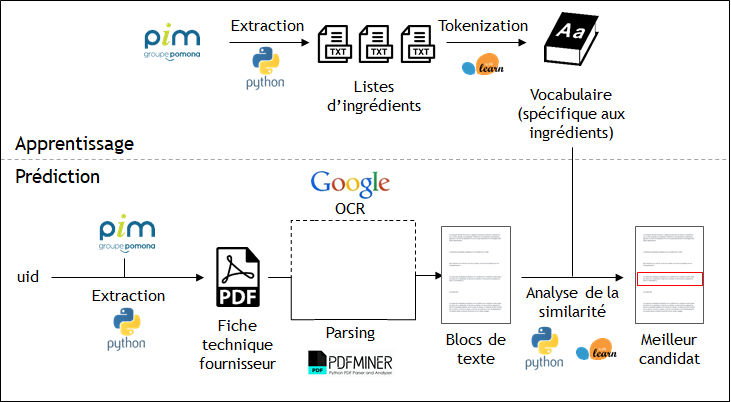
\includegraphics[width=0.9\linewidth]{img/open_model.png}
        \end{center}
        \caption{Schéma de principe du \og modèle ouvert \fg}
        \label{fig:open_model}
    \end{figure}     


        \section{Extraction des données}

        Ne garder que produits d'épicerie et boissons non alcoolisées

        \section{Conversion en blocs de texte}

        On utilise la bibliothèque PDFMiner.six. 
        Elle nous sort un long string qui contient le texte entier du document.
        On applique une \og bête \fg fonction : on splitte ce string quand on observe 2 retours à la lignes consécutifs.
        Le code est présenté en annexe.
        Pour le moment, vu la proportion importante de PDF dont le contenu est extractible

        \section{Train/Test split}

        On fait un split 50/50, on se base sur les uid pour identifier les produits.
        Sur le train set, on récupère les listes d'ingrédients du PIM.

        \section{Entrainement du modèle}

        L'entraînement est basique : on constitue seulement un vocabulaire en utilisant la fonctionnalité mise à disposition dans scikit-learn.

        \section{Calcul de la similarité}

        On calcule la similarité cosinus entre chacun des blocs, et le vocabulaire.
        On prend, systématiquement l'argmax de la similarité qu'on propose comme liste d'ingrédients.

        \section{Illustration des résultats obtenus}
    
        Mettre ici les résultats sur quelques fiches techniques présentées en annexe.
        Spoiler : rien que comme ça, les résultats sont encourageants.

        \section{Pistes d'améliorations identifiées}

        En plus de la mesure de la performance, qui est indispensable avant de pouvoir procéder à des ajustements.
        Pistes identifiées : 
        \begin{itemize}
            \item Faire un découpage du gros texte en blocs plus malin, potentiellement avec des expressions régulières
            \item Faire des \og ngrams de blocs \og, ce qui permettrait de parfois fusionner des blocs qui ont été séparés (car contenaient des retours à la ligne successifs)
            \item Essayer une autre manière de calculer la similarité ?
        \end{itemize}

    \chapter{Utilisation des données manuellement étiquetées}

    Expliciter pourquoi on ne peut pas faire tourner (référence parties précédentes) sur les listes d'ingrédients déjà présentes dans le PIM => soucis de qualité de données source. 
    Si on entraîne sur des données de mauvaise qualité, on aura de mauvais résultats.
    Le code de cette partie est présenté en annexe.    
    Le fonctionnement de ce modèle est présentés à la \reffig{fig:ground_truth_model}.
    
    \begin{figure}[htbp]
        \begin{center}
        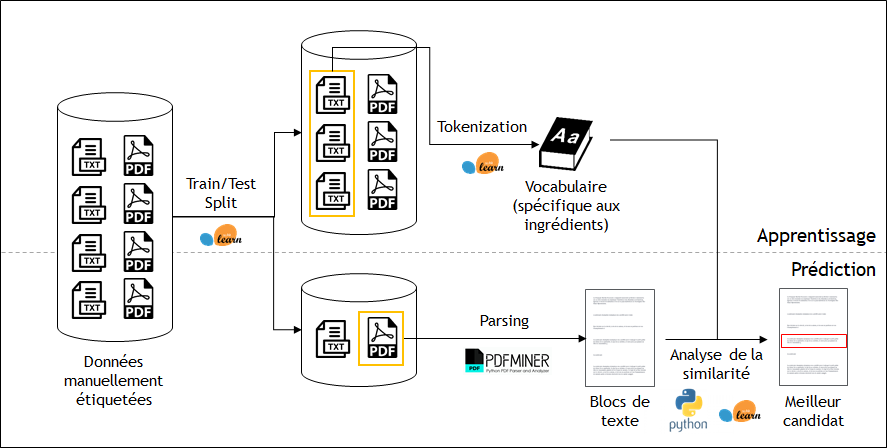
\includegraphics[width=0.9\linewidth]{img/ground_truth_model.png}
        \end{center}
        \caption{Schéma de principe du \og modèle ouvert \fg}
        \label{fig:ground_truth_model}
    \end{figure}     


        \section{Chargement des données manuellement étiquetées}

        Un bon vieux read\_csv des familles.

        \section{Train/Test split}

        Vu qu'on a moins de données, on fait train = 400 et test = 100

        \section{Entraînement du modèle}

        On fait tourner de la même manière que sur le modèle dit \og ouvert \fg

        \section{Illustration des prédictions obtenues}


    \chapter{Mesure de la performance}
    
        \section{Précision}
            \subsection{Approche naïve}

            \subsection{Avec du \og text-postprocessing \fg}
        
        \section{Similarité cosinus}

        \section{Fonction de \emph{loss} spécifique}

        Expliciter les diverses distances, et pourquoi certaines sont plus pertinentes que d'autres.

        Ex : on ne garde pas la distance de Hamming
            \subsection{Distance de Levenshtein}

            \subsection{Distance de Dameray-Levenshtein}

            \subsection{Distance de Jaro}

            \subsection{Distance de Jaro-Wrinkler}
    
        \section{Cross-validation des modèles précédents}
            
            \subsection{Modèle \og ouvert \fg}

            \subsection{Modèle entraîné sur les données étiquetées manuellement}

    \chapter{Transfer learning}
        
        \section{Principe du pré-entraînement}
        
        Expliquer qu'il s'agit d'une approche hybride des 2 modèles précédents

        \section{Illustration de l'impact sur la performance}


    \chapter{Hyperparameter tuning}
            
        \section{Les paramètres ajustables}

        \section{Application d'une grid search}